\documentclass{standalone}
\usepackage{tikz}
\usepackage{amsmath,dsfont}
\usetikzlibrary{arrows.meta, positioning, shapes.geometric, calc,patterns,quotes,decorations.pathreplacing}
\begin{document}
	
	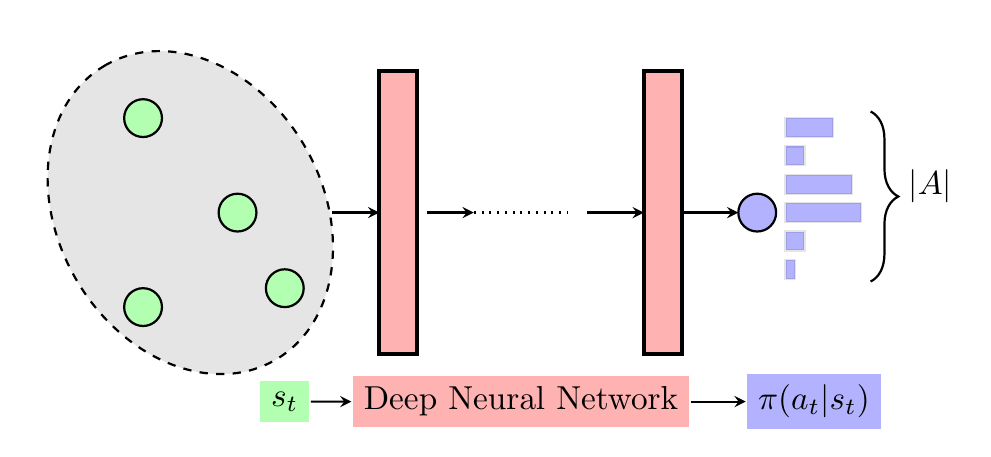
\begin{tikzpicture}[
		thick,scale=1.2, every node/.style={scale=1.2},
		state/.style={draw,circle,pattern=north east lines, pattern color=yellow,radius=0.2},
		action/.style={draw,rectangle, ,pattern=north west lines, pattern color=green}
		]
		
		% Input node (dashed ellipse)
		\draw[dashed,rotate around={120:(-3,0)},fill = black!10] (-3, 0) ellipse (1.8 and 1.4);
		
		
		\filldraw[fill=green!30] (-3.5,1) circle [radius=0.2];
		\filldraw[fill=green!30] (-3.5,-1) circle [radius=0.2];
		\filldraw[fill=green!30] (-2.5,0) circle [radius=0.2];
		\filldraw[fill=green!30] (-2,-0.8) circle [radius=0.2];
		% Hidden layers (rectangles)
		\draw[fill=red!30,line width=0.5mm] (-1,1.5) rectangle (-0.6,-1.5);
		\draw[fill=red!30,line width=0.5mm] (1.8,1.5) rectangle (2.2,-1.5);
		
		% Arrows between layers
		\draw[->,>=stealth,thick] (-1.5,0) -- (-1,0);
		\draw[->,>=stealth,thick] (-0.5,0) -- (0,0);
		\draw[->,>=stealth,thick] (1.2,0) -- (1.8,0);
		\draw[->,>=stealth,thick] (2.2,0) -- (2.8,0);
		
		
		
		% Dotted line between layers
		\draw[dotted,thick] (0,0) -- (1,0);
		
		% Output arrows
	%	\foreach \y in {1.0, 0.5, -0.5, -1.0}
	%	\draw[->,>=stealth,thick] (2.2,0) -- (3,\y);
		\filldraw[fill=blue!30] (3,0) circle [radius=0.2];
		% Output circles
	%	\foreach \y in {1.0, 0.5, -0.5, -1.0}
	%	\filldraw[fill=blue!30] (3.2,\y) circle [radius=0.2];
		
		% Output label
	%	\node at (3.2, 0.1) {$\vdots$};
		\draw [thick, decorate,decoration={brace,amplitude=10pt},yshift=2pt] (4.2,1) -- (4.2,-0.8) node [black,midway,xshift = 18pt,yshift=3pt] {$|\mathds{A}|$};
		% different probabilities
		\draw[fill=blue!30,draw opacity=0.1] (3.3,1) rectangle ++(0.5,-0.2);
		\draw[fill=blue!30,draw opacity=0.1] (3.3,0.7) rectangle++(0.2,-0.2);
		\draw[fill=blue!30,draw opacity=0.1] (3.3,0.4) rectangle++(0.7,-0.2);
		\draw[fill=blue!30,draw opacity=0.1] (3.3,0.1) rectangle ++(0.8,-0.2);
		\draw[fill=blue!30,draw opacity=0.1] (3.3,-0.2) rectangle ++(0.2,-0.2);
		\draw[fill=blue!30,draw opacity=0.1] (3.3,-0.5) rectangle ++(0.1,-0.2);
		% Network label
		\node [fill = green!30] at (-2,-2) (st){$s_t$};
		
		\node [fill = red!30] at (0.5, -2)(NN) {Deep Neural Network};
		
		% Q-function label
		\node [fill = blue!30] at (3.6, -2)(Q) {$\pi(a_t|s_t)$};
		\draw[->,>=stealth,thick](st)--(NN);
		\draw[->,>=stealth,thick](NN.east)--(Q.west);
	\end{tikzpicture}
	
\end{document}
